%% inicio, la clase del documento es especificacion.cls
\documentclass{manual}
\usepackage[onelanguage, commentsnumbered, linesnumbered, boxed, ruled]{algorithm2e}
\usepackage{pdfpages}
\usepackage{amsfonts}
\usepackage{amssymb}
\usepackage{array}
\usepackage{longtable}
\usepackage{float}
\usepackage{setspace}
\usepackage{listings}
\usepackage[linktocpage, hidelinks]{hyperref}
\lstset{ %
    language=Java, % lenguaje
    basicstyle=\bfseries\ttfamily,
    keywordstyle=\color{blue},
    commentstyle=\color{brown},
    backgroundcolor=\color{gray!10},
    showstringspaces=false
}

%% datos generales y para la tapa
\titulo{Manual de usuario}
\subtitulo{JHawanet Framework}
\author{Gabriel Gonzalo Alexander Sanhueza Fuentes}


%% inicio de documento
\begin{document}

%% crea la tapa
\maketitle

\adddevelopment{Gabriel Sanhueza Fuentes}{Administrador, Analista, Dise�ador, Implementador y Tester.}{gsanhueza15@alumnos~.utalca.cl}

\addcounterpart{Jimmy H. Guti�rrez-Bahamondes}{Cliente/Profesor gu�a}{}
\addcounterpart{Jimmy H. Guti�rrez-Bahamondes}{Cliente/Profesor co-gu�a}{}

\addrevision{1}{23/06/2020}{Primer borrador}
\addrevision{1.1}{04/07/2020}{Reescrito manual usando latex}

\RevisionHistoryPage


%% indices
\tableofcontents
\listoffigures
%\listoftables

%% abstract

%WRITE HERE
\section{Como agregar un nuevo algoritmo}
Para agregar un nuevo algoritmo a la aplicaci�n se debe implementar la interfaz \textit{Algorithm}. En la Figura \ref{fig:metaheuristics} se puede ver la interfaz correspondiente.

\begin{figure}[H]
    \centering
    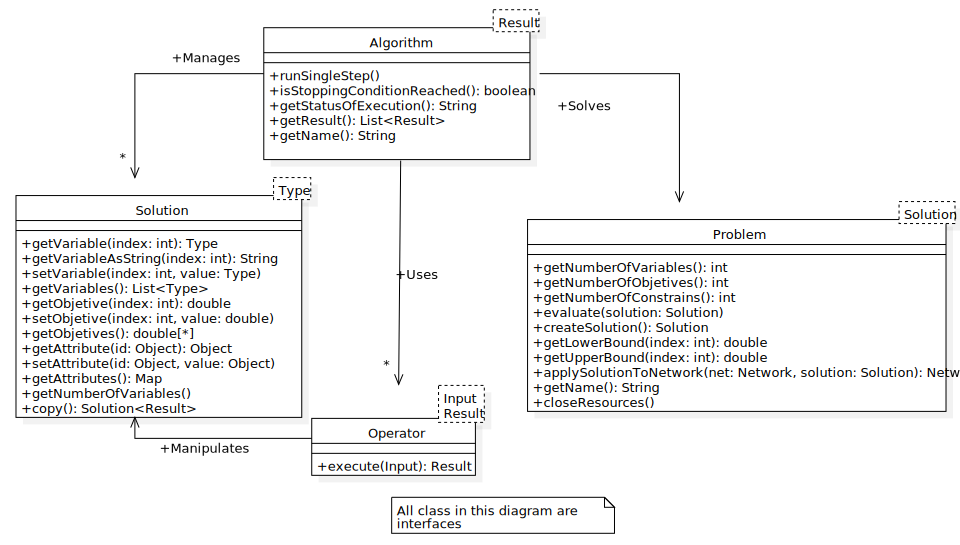
\includegraphics[width=\textwidth]{Seccion1/assets/d_class_metaheuristics}
    \caption{Diagrama de clases del m�dulo de metaheur�sticas.}
    \label{fig:metaheuristics}
\end{figure}

Esta interfaz cuenta con los siguientes m�todos:
\begin{itemize}
    \item \textit{RunSingleStep}: Este m�todo debe ejecutar un �nico paso del algoritmo (Una sola generaci�n/iteraci�n). 
    \item \textit{isStoppingConditionReached}: Este m�todo indica si la condici�n de t�rmino del algoritmo ha sido alcanzada. 
    \item \textit{getStatusOfExecution}: Este m�todo puede devolver un \textit{String} con informaci�n del algoritmo como se muestra en la Figura \ref{fig:getStatusOfExecution} y \ref{fig:getStatusOfExecution2}.
    \item \textit{getResult}: Devuelve el resultado del algoritmo.
    \item \textit{getName}: Devuelve el nombre del algoritmo.
\end{itemize}

\begin{figure}[H]
    \centering
    \includegraphics[width=0.5\textwidth]{Seccion1/assets/SingleObjectiveRunningWindow.png}
    \caption[Mensaje retornado por el m�todo \textit{getStatusOfExecution} en la ventana monoobjetivo.]{Mensaje retornado por el m�todo \textit{getStatusOfExecution} en la ventana monoobjetivo (Est� indicado por la flecha roja).}
    \label{fig:getStatusOfExecution}
\end{figure}

\begin{figure}[H]
    \centering
    \includegraphics[width=0.5\textwidth]{Seccion1/assets/MultiObjectiveRunningWindow.png}
    \caption[Mensaje retornado por el m�todo \textit{getStatusOfExecution} en la ventana multiobjetivo.]{Mensaje retornado por el m�todo \textit{getStatusOfExecution} en la ventana multiobjetivo (Est� indicado por la flecha roja).}
    \label{fig:getStatusOfExecution2}
\end{figure}

Para llevar a cabo la simulaci�n, la aplicaci�n llama al m�todo \textit{RunSingleStep} hasta que \textit{isStoppingConditionReached} sea verdadero. Adicionalmente, dentro del mismo m�todo \textit{RunSingleStep} tambi�n se deber�a asegurar que una vez sea alcanzada la condici�n de termino no se realicen nuevas operaciones. Un ejemplo de \textit{RunSingleStep} utilizado en el Algoritmo NSGAII y GA se puede ver en la Figura \ref{fig:runASingleStep}.
 
\begin{figure}[H]
    \centering
    \includegraphics[width=\textwidth]{Seccion1/assets/runASingleStep.png}
    \caption{M�todo \textit{runASingleStep} para los algoritmos evolutivos.}
    \label{fig:runASingleStep}
\end{figure}


\section{Como agregar un nuevo problema}

Para agregar un nuevo problema se debe implementar la interfaz \textit{Problem} que se muestra en la Figura \ref{fig:metaheuristics}.  Esta interfaz posee los siguientes m�todos:

\begin{itemize}
    \item \textit{getNumberOfVariables}: Indica el n�mero de variables del problema.
    \item \textit{getNumberOfObjectives}: Indica el n�mero de objetivos del problema.
    \item \textit{getNumberOfConstrains}: Indica el n�mero de restricciones del problema.
    \item \textit{evaluate}: Eval�a una soluci�n y sus restricciones.
    \item \textit{createSolution}: Crea una nueva soluci�n para el problema.
    \item \textit{getLowerBound}: Indica el valor m�nimo que puede tomar una variable en un �ndice espec�fico.
    \item \textit{getUpperBound}: Indica el valor m�ximo que puede tomar una variable en un �ndice espec�fico.
    \item \textit{applySolutionToNetwork}: Toma una soluci�n y la aplica sobre una red (Instancia de \textit{Network} que posteriormente puede ser guardada como un archivo inp). Este m�todo es opcional y en caso de que no est� implementado devuelve el valor \textit{null}. Se puede ver un ejemplo de este m�todo en la Figura \ref{fig:applySolutionToNetwork}. Este m�todo es llamado por la aplicaci�n cuando se selecciona una soluci�n en la pesta�a de resultados y se presiona el bot�n guardar como inp.
    \item \textit{getName}:  El nombre del problema.
    \item \textit{closeResources}: Cierra los recursos usado por el problema. Generalmente, el �nico recurso a cerrar ser�a el simulador hidr�ulico EpanetAPI. Implementar este m�todo es opcional. Este m�todo es llamado por la aplicaci�n cuando se termina el experimento.
\end{itemize}

\begin{figure}[H]
    \centering
    \includegraphics[width=\textwidth]{Seccion2/assets/applySolutionToNetwork.png}
    \caption{Ejemplo del m�todo \textit{applySolutionToNetwork}.}
    \label{fig:applySolutionToNetwork}
\end{figure}

\section{Como agregar un nuevo operador}

Para crear un nuevo operador se debe implementar la interfaz \textit{Operator} o alguna de sus subinterfaces o subclases. Esta interfaz cuenta con un �nico m�todo. La interfaz se muestra en la Figura \ref{fig:metaheuristics}. El m�todo de la interfaz es:
\begin{itemize}
    \item execute: M�todo que realiza una operaci�n sobre un operando y devuelve un objeto resultante de dicha operaci�n. Generalmente, este m�todo realiza una acci�n sobre una soluci�n o una lista de soluciones y retorna la soluci�n resultante de la operaci�n realizada.
\end{itemize}

Para configurar los par�metros del operador desde la ventana de configuraci�n, debe haber un constructor p�blico que posea la anotaci�n \textit{@DefaultConstructor}.

\subsection{\textit{@DefaultConstructor}}

La anotaci�n \textit{@DefaultConstructor} indica el constructor que debe ser usado al momento de crear una instancia del operador. Esta anotaci�n recibe un arreglo de \textit{NumberInput}, el cual se define en la siguiente secci�n. El arreglo debe tener la misma cantidad de argumentos que los par�metros del constructor como se muestra en la Figura \ref{fig:constructor_un_parametro} y Figura \ref{fig:constructor_multi_parametro}. 

\begin{figure}[H]
    \centering
    \includegraphics[width=\textwidth]{Seccion3/assets/ConstructorUnParametro.png}
    \caption{Constructor de un solo par�metro.}
    \label{fig:constructor_un_parametro}
\end{figure}
  
\begin{figure}[H]
    \centering
    \includegraphics[width=\textwidth]{Seccion3/assets/ConstructorMultiParametro.png}
    \caption{Constructor de un solo par�metro.}
    \label{fig:constructor_multi_parametro}
\end{figure}

Esta anotaci�n solo puede ser usada en un �nico constructor por clase. Usar esta anotaci�n en m�s de un constructor lanzara una excepci�n en tiempo de ejecuci�n. Adicionalmente, el constructor que use esta anotaci�n solo puede tener par�metros de tipo \textit{int} o \textit{double}.

La interfaz gr�fica creada para cada anotaci�n se puede ver en la Figura \ref{fig:interfaz_uniform_selection} y \ref{fig:interfaz_polynomial_mutation}.

\begin{figure}[H]
    \centering
    \includegraphics[width=0.5\textwidth]{Seccion3/assets/InterfazConfiguracionUniformSelection.png}
    \caption{Interfaz para configurar el operador \textit{UniformSelection}.}
    \label{fig:interfaz_uniform_selection}
\end{figure} 
 
\begin{figure}[H]
    \centering
    \includegraphics[width=0.5\textwidth]{Seccion3/assets/InterfazConfiguracionIntegerPolynomialMutation.png}
    \caption{Interfaz para configurar el operador \textit{IntegerPolynomialMutation}.}
    \label{fig:interfaz_polynomial_mutation}
\end{figure}

La anotaci�n puede tener un arreglo vac�o, lo cual indica que el constructor no recibir� par�metros.

\section{Como agregar un nuevo experimento y hacerlo visible desde la interfaz gr�fica}

Un experimento es una clase que contiene una lista de algoritmos para resolver un problema espec�fico. Los algoritmos que conforman el experimento deben ser de un mismo tipo, por ejemplo, que la lista tenga instancias ``n'' repeticiones del Algoritmo Gen�tico. Actuando ``n'' como el n�mero de ejecuciones independientes del algoritmo. En la Figura \ref{fig:metaheuristics_extendido}, se muestra las interfaces del m�dulo de metaheur�sticas extendido.

\begin{figure}[H]
    \centering
    \includegraphics[width=\textwidth]{Seccion4/assets/d_class_metaheuristics_extendido.eps}
    \caption{Diagrama m�dulo metaheur�stica extendido.}
    \label{fig:metaheuristics_extendido}
\end{figure}

Para crear el experimento la aplicaci�n cuenta con una clase llamada \textit{ExperimentBuilder}.
Los par�metros \textit{ExperimentBaseDirectory} y \textit{ReferenceFrontDirectory} solo tienen uso en experimentos multiobjetivos. \textit{ExperimentBaseDirectory} indica donde guardar la frontera de Pareto de cada repetici�n del algoritmo multiobjetivo. En cambio, \textit{ReferenceFrontDirectory} indica donde guardar la frontera de Pareto final, que se obtiene al unir las fronteras de cada repetici�n y extraer solamente las soluciones no dominadas de dicho conjunto. 

\section{Interfaz Registrable}

Esta interfaz declara el m�todo \textit{build} y \textit{getParameters}. La declaraci�n del m�todo \textit{build}  corresponde a la siguiente:

\begin{lstlisting}
    R build(String inpPath) throws Exception;
\end{lstlisting}

Donde R corresponde al tipo de valor devuelto por la funci�n.

De esta clase se heredan dos subinterfaces. La primera corresponde a \textit{SingleObjectiveRegistrable} que debe ser usada para implementar los problemas monoobjetivos. En cuanto a la segunda, esta corresponde a \textit{MultiObjectiveRegistrable}, la cual se debe usar para los problemas multiobjetivos. El m�todo build sobreescrito por estas clases tiene la siguiente asignatura: 

\begin{lstlisting}
    Experiment<?> build(String inpPath) throws Exception;
\end{lstlisting}

\noindent %% remueve la identaci�n
donde Experiment consiste en una clase que almacena una lista de algoritmos (Del mismo tipo) y el problema a resolver por estos algoritmos.

Las nuevas clases deben implementar la interfaz \textit{SingleObjectiveRegistrable} o \textit{MultiObjectiveRegistrable}, dependiendo del tipo de problema a tratar. Las clases que implementen cualquiera de estas dos interfaces deben ser guardados en una estructura de datos, la cual ser� recorrida cuando se inicie la ejecuci�n del programa y analizada usando la \textit{Java Reflection API}. Este an�lisis consistir� en escanear y validar el cumplimiento de la convenci�n establecida para las clases que implementan est� interfaz. Esta convenci�n consiste en lo siguiente:

\begin{itemize}
    \item La clase debe contener un �nico constructor que use la anotaci�n \textit{@NewProblem.}
    \item Si el constructor requiere par�metros �stos deben estar descritos usando la anotaci�n \textit{@Parameters.}
    \item El constructor debe declarar los par�metros en el siguiente orden, de acuerdo con su tipo.
    \begin{enumerate}
        \item Object: Usado para inyectar los operadores. �stos pueden posteriormente ser casteados a su tipo correcto. La anotaci�n correspondiente es \textit{@OperatorInput}
        \item File: Usados cuando el problema requiere informaci�n adicional que se encuentra en un archivo diferente. La anotaci�n correspondiente es \textit{@FileInput}
        \item int, Integer, double o Double: Usado generalmente para configurar valores en el algoritmo o si el problema requiere otros valores que no fueron solicitados al crear los operadores. Las anotaciones correspondientes son \textit{@NumberInput y @NumberToggleInput.}
        \item El constructor debe solicitar la misma cantidad de par�metros que las descritas en la anotaci�n \textit{@Parameters.}
    \end{enumerate}
\end{itemize}

Si estas convenciones no se cumplen, entonces un error en tiempo de compilaci�n ser� emitido como se mencion� anteriormente en la secci�n anterior.

El orden en el que son inyectados los par�metros consiste en el siguiente:

\begin{enumerate}
    \item Par�metros descritos por \textit{@OperatorInput}
    \item Par�metros descritos por \textit{@FileInput}
    \item Par�metros descritos por \textit{@NumberInput}
    \item Par�metros descritos por \textit{@NumberToggleInput}
\end{enumerate}

Una vez que se haya configurado el problema a trav�s de la interfaz se crear� la instancia de la clase que hereda de Registrable y se llamar� a su m�todo build, para crear el experimento y comenzar su ejecuci�n.

La estructura de datos para registrar las clases que heredan de \textit{SingleObjectiveRegistrable} y \textit{MultiObjectiveRegistrable} se encontrar� en la clase \textit{RegistrableConfiguration}.


A continuaci�n de define detalladamente cada una de las anotaciones permitidas en la clase Registrable.

\input{Seccion4/anotaciones_registrable}

%% ambiente glosario
\begin{glosario}
 \item[RDA] Este es el significado del primer t�rmino, realmente no se bien lo que significa pero podr�a haberlo averiguado si hubiese tenido un poco mas de tiempo.
 \item[GA] Este si se lo que significa pero me da lata escribirlo...
\end{glosario}


%% genera las referencias
\bibliography{refs}

\end{document}

   

